% This is the file where my Master Thesis will be written. It uses the adapted
% LNCS Template.
%
% I'll be using a few codes in the comments, which can be easily looked up:
% * NOTE: theseis-text related comments
% * TODO: thesis-related TODO's
% * WARN: latex/formatting-related warningss
%
% WARN: for running head, subsititute the line below by:
% \documentclass[runningheads,a4paper]{llncs}
\documentclass{llncs}

% \usepackage{geometry}
% \geometry{
%  a4paper,         % or letterpaper
%  textwidth=15cm,  % llncs has 12.2cm
%  textheight=24cm, % llncs has 19.3cm
%  heightrounded,   % integer number of lines
%  hratio=1:1,      % horizontally centered
%  vratio=2:3,      % not vertically centered
%}
%
%%% WARN: custom extension
\usepackage{xcolor}
\newcommand{\todo}[1]{\textcolor{red}{TODO: #1}\PackageWarning{TODO:}{#1!}}

%%% GLOSSARIES
\usepackage{glossaries}

%%% inline code
\usepackage{xparse}
\NewDocumentCommand{\codeword}{v}{%
\texttt{\textcolor{blue}{#1}}%
}

%%% figures
\usepackage{graphicx}
\usepackage{wrapfig}

%%% tables
\usepackage{booktabs}

\usepackage{amssymb}

\usepackage{url}
\def\UrlBreaks{\do\/\do-}


\makeglossaries

\newacronym{tls}{TLS}{Transport Layer Security}%
\newacronym{ssl}{SSL}{Secure Sockets Layer}%
\newacronym{ietf}{IETF}{Internet Engineering Task Force}%
\newacronym{mac}{MAC}{Message Authentication Code}%
\newacronym{psk}{PSK}{Pre-Shared Key}%
\newacronym{rpk}{RPK}{Raw Public Key}%
\newacronym{aead}{AEAD}{Authenticated Encryption With Associated Data}%
\newacronym{pkc}{PKC}{Public Key Cryptography}%
\newacronym{hkdf}{HKDF}{HMAC-based Extract-and-Expand Key Derivation Function}%
\newacronym{html}{HTML}{Hypertext Markup Language}%
\newacronym{https}{HTTPS}{Hypertext Transfer Protocol Secure}%
\newacronym{ecc}{ECC}{Elliptic Curve Cryptography}%
\newacronym{iv}{IV}{Initialization Vector}%
\newacronym{ecdh}{ECDH}{Elliptic Curve Diffie-Hellman}%
\newacronym{ecdhe}{ECDHE}{Elliptic Curve Diffie-Hellman Ephemeral}%
\newacronym{ecdsa}{ECDSA}{Elliptic Curve Digital Signature Algorithm}%
\newacronym{rfc}{RFC}{Request For Comment}%
\newacronym{prf}{PRF}{Pseudo-Random Function}%
\newacronym{rsa}{RSA}{Rivest-Shamir-Adleman}%
\newacronym{dh}{DH}{Diffie-Hellman}%
\newacronym{pms}{PMS}{premaster secret}%
\newacronym{pubk}{PubK}{Public Key}%
\newacronym{privk}{PrivK}{Private Key}%
\newacronym{dsa}{DSA}{Private Key}%
\newacronym{pfs}{PFS}{Perfect Forward Secrecy}%
\newacronym{mitm}{MITM}{Man In The Middle}%
\newacronym{ac}{AC}{Asymmetrical Cryptography}%
\newacronym{sc}{SC}{Symmetrical Cryptography}%
\newacronym{iot}{IoT}{Internet Of Things}%
\newacronym{dtls}{DTLS}{Datagram TLS}%
\newacronym{coap}{CoAP}{Constrained Application Protocol}%
\newacronym{ec}{EC}{Elliptic Curve}%
\newacronym{sca}{SCA}{Side-Channel Attack}%
\newacronym{ocsp}{OCSP}{Online Certificate Status Protocol}
\newacronym{crl}{CRL}{Certificate Revocation List}
\newacronym{ca}{CA}{Certification Authority}
\newacronym{sni}{SNI}{Server Name Indication}
\newacronym{dos}{DoS}{Denial-of-Service}
\newacronym{ddos}{DDoS}{Distributed Denial-Of-Service}
\newacronym{pki}{PKI}{Public Key Infrastructure}
\newacronym{ae}{AE}{Authenticated Encryption}
\newacronym{nsa}{NSA}{US National Security Agency}


%%% WARN: added as specified here:
% https://tex.stackexchange.com/questions/272200/table-of-contents-showing-the-title-as-only-entry-latex
\setcounter{tocdepth}{2}
\makeatletter
\renewcommand*\l@author[2]{} % removes author name from TOC
\renewcommand*\l@title[2]{} % removes title name from TOC
\makeatletter
%%%
%
\usepackage{makeidx}  % allows for indexgeneration
%
\begin{document}
%
\frontmatter          % for the preliminaries
%
\pagestyle{headings}  % switches on printing of running heads
%
\addtocmark{TLS For IoT} % additional mark in the TOC

\tableofcontents
\newpage

\mainmatter              % start of the contributions
%
\title{Transport Layer Security Protocol For Internet Of Things}
%
\titlerunning{TLS For IoT}  % abbreviated title (for running head)
%                                     also used for the TOC unless
%                                     \toctitle is used
%
\author{{Illya Gerasymchuk} \\
\email{illya.gerasymchuk@tecnico.uliboa.pt},\\ WWW home page:
\texttt{https://iluxonchik.github.io/}}
%
\authorrunning{Illya Gerasymchuk} % abbreviated author list (for running head)
%
%%%% list of authors for the TOC (use if author list has to be modified)
\tocauthor{Illya Gerasymchuk}
%
\institute{Instituto Superior Técnico}
% WARN: supper hacked-in
\supervisors{Ricardo Chaves, Aleksandar Ilic}
\maketitle              % typeset the title of the contribution

\begin{abstract}
This paper explores the idea of developing a lightweight \gls{tls} protocol
for the \gls{iot}. It begins by explaining why there is a need for security in
the \gls{iot} ecosystem and why \gls{tls}, as it is, cannot be used in most cases,
due to the constrained nature of many \gls{iot} devices. Next, the state
of the art in the area is described, most of which is done for \gls{dtls}, but can
also be applied to \gls{tls}, since \gls{dtls} is just an adaptation of
\gls{tls} for unreliable transport protocols, such as UDP. The document proceeds with a
summary of \gls{tls} 1.2, outline its main differences from \gls{tls} 1.3
and give an overview of the how \gls{dtls} differs from \gls{tls}. Finally, the architecture of the solution that will be developed, which relies
heavily on the use of the \gls{tls} extension mechanism, is presented.

\keywords{TLS, DTLS, SSL, IoT, cryptography, protocol, lightweight cryptography}
\end{abstract}
%
\section{Intoduction}
%

The \gls{iot} is a network of devices, from simple sensors to smartphones and wearables
that are connected together. In fact, it can be any other object that has an assigned
IP address and is provided with the ability to transfer data over a network. Even
something such as a salt shaker\cite{SMALTThe76:online} can now be part of the global network.

The \gls{iot} technology can be used solve problems and make our lives easier,
unfortunately, however, its technological development tends to focus on
innovative design rather than on privacy and security. \gls{iot} devices frequently
connect to networks using inadequate security and are hard to update when
vulnerabilities are found.

This lack of security in the \gls{iot} ecosystem has been exploited by the
the \textit{Mirai} botnet\cite{sec17ant94:online} when it overwhelmed several high-profile
targets with massive \gls{ddos} attacks. This is the most devastating attack involving \gls{iot}
devices done to date, the \textit{Reaper} botnet\cite{ReaperCa10:online}, however, could be
even more devastating if it is ever put to malicious use. Others will inadvertently
come in the future. \textit{SecurityNow}\cite{GRCSecur72:online} is a weekly podcast
centered around computer security and the topics that surround it. I have been a regular listener
since $2012$ and noticed a clear trend: as the time goes on, the lack of
security of \gls{iot} devices, as well as various problems caused by it, from
the compromise of privacy, to the massive \gls{ddos} attacks is a topic that comes up
more and more often. In fact, now it is mentioned almost every week.

\gls{tls} is the most used security protocol in the world and it allows two peers
to communicate securely. It is designed to run on top of a reliable, connection-oriented
protocol, such as TCP. \gls{dtls} is the version of \gls{tls} that runs on top
of an unreliable transport protocol, such as UDP. Most \gls{iot} devices have
very limited processing power, storage and energy. Moreover, the performance of
TCP is known to be inefficient in wireless networks, due to its congestion control
algorithm and this situation is worsened with the low-power radios and lossy
links found in sensor networks. Therefore, \gls{dtls}, which runs on top
of UDP, is used more frequently in such devices. The work that will be done in the context of this dissertation, can however,
be applied to either one of them, so even though mostly
\gls{tls} will be mentioned, almost everything also applies to \gls{dtls} as well, since it is just
an adaption of \gls{tls} over unreliable transport protocols, with no changes done
the core protocol.

The problem in using (D)\gls{tls} in \gls{iot} is that it is not lightweight, since
it was not designed for such environments. An \gls{iot} device may only have
$256$ KB of RAM and needs to conserve the battery, while sending and receiving
a large amount of small information constantly. For example, imagine a temperature sensor
that sends the temperature measures every $30$ seconds to a server. In this case
it just needs to send a few bytes of data and do it with minimal overhead, to conserve
RAM and battery. If that sensor is going to use (D)\gls{tls} $1.2$, it will need
two extra roundtrips before it can send any data, which can be an extra hundreds of
milliseconds. Besides that, it will need to perform heavy mathematical operations
involved in cryptography, using even more battery and taking even more time.
There is a clear need for a more lightweight (D)\gls{tls} for the \gls{iot}.

The goal of this work is to develop a lightweight version of (D)\gls{tls} that is
fully backwards compatible and does not require any third-party entities, in order
to minimize the friction of adoption. The solution will be developed for
(D)\gls{tls} versions $1.2$ and $1.3$. The idea is to make it customizable,
depending on the security requirements of the context of its use, in that sense, it is similar to a framework.

In the process of my work on this dissertation, I have made several
contributions to the \gls{tls} $1.3$ specification and have been officially
recognized as a contributor, my name will be on the final document specifying
the \gls{tls} $1.3$ protocol.

The document is organized as follows: Section 2 describes the background. It
begins with introducing some of the concepts that will be used throughout
the document, after which it describes the \gls{tls} and \gls{dtls} protocol
versions $1.2$ and $1.3$, with a focus on the version $1.2$ since
it is the latest and the most used version of the protocol (version $1.3$ is still in
draft mode). Section 3 describes all of the related work done in the area and
the current state of the art. Finally, Section 4 provides an architecture of the
solution that will be developed in the second part of the dissertation,
an explanation of how the results will be evaluated, a general work plan
and a conclusion of the work done in this part.

\section{Background}

\subsection{Symmetric vs Asymmetric Cryptography}

\gls{ac} is more expensive than \gls{sc} in terms of performance. This is mainly due
to two facts: larger key sizes are required for an \gls{ac} system to achieve the
same level of security as in a \gls{sc} system  and \codeword{CPU}s are slower at performing the underlying
mathematical operations involved in \gls{ac}, namely exponentiation requires
$O(log e)$ multiplications for an exponent $e$. For example,
the 2016 \codeword{NIST} report \cite{Recommen44:online}
suggests that an \gls{ac} algorithm would need to use a secret key with size of \codeword{15360 bits}
to have equivalent security to a \codeword{256-bit} secret key for a \gls{sc} algorithm.
This situation is ameliorated by \gls{ecc}, which requires keys of \codeword{512 bits}, but
it is still slower than using \gls{sc}. The 2017 \codeword{BSI} report \cite{Kryptogr1:online} (from the
German federal office for information security) suggests similar numbers.

Another argument for avoiding as much as possible the use of \gls{ac}
algorithms is that they require additional storage space and this might be a problem for some \gls{iot} devices,
like \codeword{class 1} devices according to the terminology of constrained-code
networks\cite{RFC7228} which have approximately \codeword{10KB} of RAM and \codeword{100KB}
of persistent memory. I measured and compared the resulting size of the complied \textit{mbedTLS 2.6.0} library
\cite{SSLLibra13:online} when it was with and without the \codeword{RSA} module
(located in the \codeword{rsa.c} file). The conclusion is that that using the \codeword{rsa.c} module adds an extra of \codeword{32KB}.

\subsection{Public Certificates and Certificate Chains}

A public key certificate, also known as a digital certificate, is an electronic
document used to prove the ownership of a \gls{pubk}. This allows the other parties
to rely upon assertions made by the \gls{privk} that corresponds to the \gls{pubk}
that is certified. In the context of (D)\gls{tls}, certificates serve as a guarantee
that the communication is done with the claimed entity and not someone impersonating it.

A \gls{ca} is an entity that issues digital certificates. There are two types of
\gls{ca}s: the \textbf{root \gls{ca}s} and the \textbf{intermediate \gls{ca}s}.
An intermediate \gls{ca} is provided with a certificate with signing capabilities
signed by one of the root \gls{ca}s. A \textbf{certificate chain} is a list of
certificates from the root certificate to the end-user certificate, including
any intermediate certificates along the way. In order for a certificate
to be trusted by a device, it must be issued by a \gls{ca} that is included in that device's trusted store.

In (D)\gls{tls}, the certificates are in the \codeword{X.509} format, which is
described in \codeword{RFC 5280}\cite{rfc5280}.

\subsection{AEAD Ciphers}

\gls{ae} and \gls{aead} are forms of encryption which simultaneously provide
confidentiality, integrity and authenticity guarantees on the data. An \gls{ae}
cipher takes as input a \codeword{key}, a \codeword{nonce} and a \codeword{plaintext}
and outputs the pair \codeword{(ciphertext, MAC)}, if it is encrypting and does the inverse
process, while also performing the \gls{mac} check if it is decrypting.

\gls{aead} is nothing more than a variant of \gls{ae}, which comes with an extra
input parameter that is additional data that is \textbf{only authenticated, but not encrypted}.
Some \gls{aead} ciphers have shorter authentication tags (\textit{i.e.} shorter \gls{mac}s),
which makes then more suitable for low-bandwidth networks, since the messages to be sent are smaller in size.

\subsection{Elliptic Curve Cryptography}

\gls{pubk} cryptography is based on the use of one-way math functions,
which are function where it is easy to compute the answer given an input,
but hard to compute the input given the answer. For example, RSA uses factoring
as the one one way function: it is easy to multiply large numbers, but it is hard
to factor them.

\gls{ecc} is based on elliptic curves, which are set of points $(x,y)$ that are
solutions to the equation $y^2 = x^3 + ax + b$, where $4a^3 + 27b^2 \neq 0$.
Depending on the value of $a$ and $b$, elliptic curves assume different shapes
on the plane.

The security of \gls{ecc} is based on the the elliptic curve discrete logarithm
problem, which states that scalar multiplication is a one way function. To exemplify,
given a curve $E(\mathbb{Z}/p\mathbb{Z})$ and points $Q$ and $P$ on that curve
$Q,P \in E(\mathbb{Z}/p\mathbb{Z})$, where $Q$ is a multiple of $P$, the elliptic curve discrete logarithm problem
states that finding the integer $k$, such that $Q=kP$ is a very hard problem.

\subsection{The TLS Protocol}

\gls{tls} is a \textbf{client-server} protocol
that runs on top a \textbf{connection-oriented and reliable transport protocol},
such as \textbf{TCP}. Its main goal is to provide \textbf{privacy} and \textbf{integrity}
between the two communicating peers. Privacy implies that a third party will not
be able to read the data, while integrity means that a third party will not be
able to alter the data.

In the TCP/IP Protocol Stack, \gls{tls} is placed between the \textbf{Transport}
and \textbf{Application} layers. it is designed to make the application developer's
life easier: all the developer has to do is create a "secure" connection, instead
of a "normal" one.

From the top-level view, in a typical connection, there are three basic steps
that \gls{tls} is responsible for:
\begin{enumerate}
  \item \textbf{negotiate security parameters} - the communicating peers agree on
  a set of security parameters to be used in a \gls{tls} connection, such as the
  algorithm used for bulk data encryption and the secret keys.
  \item \textbf{authenticate one to another} - usually only the server authenticates iself to the client.
  \item \textbf{communicate securely} - use the negotiated security parameters
  to encrypt and authenticate the data, communicating securely with each other.
\end{enumerate}


\subsubsection{SSL vs TLS: What's The Difference?}

You will find the names \gls{ssl} and \gls{tls} used interchangeably in the literature,
so it is important to distinguish both. \gls{tls} is an evolution of the \gls{ssl} protocol. The protocol changed
its name from \gls{ssl} to \gls{tls} when it was
standardized by the \gls{ietf}. \gls{ssl}
was a proprietary protocol owned by Netscape Communications, and The \gls{ietf}
decided that it was a good idea to standardize it, which resulted in \codeword{RFC 2246}\cite{RFC2246},
specifying \gls{tls} $1.0$, which was nothing more than a new version \gls{ssl} 3.0\cite{RFC6101}, very few changes were made.
%

\subsubsection{Security Services}
%
\gls{tls} provides the following security services:
\begin{itemize}
\item \textbf{authentication} - both, \textbf{peer entity} and \textbf{data origin} (or \textbf{integrity})
authentication.
\subitem \textbf{peer entity authentication} - a peer has a guarantee that it is talking to certain entity, for example, \codeword{www.google.com}.
This is achieved thought the use of \gls{ac}, also known as \gls{pkc}, (\textit{e.g.} \codeword{RSA} and \codeword{DSA})
or \textbf{symmetric key cryptography}, using a \gls{psk}.
\item \textbf{confidentiality} - the data transmitted between the communicating
entities (the client and the server) is encrypted. Symmetric cryptography is
used for data encryption (\textit{e.g.}, \codeword{AES}).
\item \textbf{integrity} (also called \textbf{data origin authentication}) - a peer can be sure that the data was not modified or forged,
\textit{i.e.}, there is a guarantee that the received data is coming from the expected entity. For example, a peer can be sure
that the \codeword{index.html} file that sent to when it connected to \codeword{www.google.com} in fact
came from \codeword{www.google.com} and that it was not tampered modified en
route by an attacker (\textbf{data integrity}). This is achieved either through the use
of a keyed \gls{mac} or an \gls{aead} cipher.
\end{itemize}

Despite using \gls{pkc}, \gls{tls} does \textbf{not} provide \textbf{non-repudiation services}:
neither \textbf{non-repudiation with proof of origin}, which addresses the peer denying
the sending of a message, not \textbf{non-repudiation with proof of delivery}, which
addresses the peer denying the receipt of a message. This is due to the fact that
instead of using \textbf{digital signatures}, either a keyed \gls{mac} or an \gls{aead}
cipher is used, both of which require a secret to be \textbf{shared} between the peers.

All of the tree security services are not required to be used in every situation.
In this sense, \gls{tls} is like a framework that allows to select which security services should be used for a communication session. As an example,
certificate validation might be skipped, which means that the \textbf{authentication} guarantee is not provided. There are some differences regarding this claim between \gls{tls} $1.2$
and \gls{tls} $1.3$, for example, while in the first you have a \codeword{null}
cipher (no authentication, no confidentiality, no integrity), in the latter
this is not true, since it deprecated all non-\gls{aead} ciphers in favor of
\gls{aead} ones.

\subsubsection{Cipher Spec vs Cipher Suite}

The meaning of these terms differs in \gls{tls} $1.2$ and \gls{tls} $1.3$. For \gls{tls} $1.2$,
\textbf{cipher spec} defines the message encryption algorithm and the message
authentication algorithm, while the \textbf{cipher suite} is the \textbf{cipher spec},
alongside the definition of the \textbf{key exchange} algorithm and the \gls{prf} (used in key generation). In \gls{tls} 1.3, the
 \textbf{cipher spec} has been removed altogether, since the  \textbf{ChangeCipherSpec}
 protocol has been removed. The concept of \textbf{cipher suite} has been updated
 to define the pair of \gls{aead} algorithm and hash function to be used with
 \gls{hkdf}: in \gls{tls} $1.3$ the  \textbf{key exchange} algorithm is negotiated via
 extensions.

\subsubsection{TLS (Sub)Protocols}

In reality \gls{tls} is composed of several protocols (illustrated in \ref{fig:tls-subprotocols}), which are briefly described below:
\begin{itemize}
  \item \textbf{\gls{tls} Record Protocol} - the lowest layer in \gls{tls}. It is
  the layer that located directly on top of \textbf{TCP/IP} and it serves as an
   \textbf{encapsulation for the remaining sub-protocols} (\codeword{4} in case of \gls{tls} 1.2
   and \codeword{3} in case of \gls{tls} 1.3). To the  \textbf{Record Protocol},
   the remaining sub-protocols are what \codeword{TCP/IP} is to \codeword{HTTP}.
   A \gls{tls} Record is comprised of 4 fields, with the first 3 comprising the
   \gls{tls} Record header: a 1-byte record \codeword{type},
   specifying the type of record that is encapsulated (ex: value \codeword{0x16}
   for the handshake protocol), a 2-byte \codeword{TLS version} field, a
   2-byte \codeword{length} field specifying the length of the data in the record, excluding
   the header itself (this means that \gls{tls} has a maximum record size
   of \codeword{16384} bytes), and a \codeword{fragment} field whose size in bytes is specified
   by the \codeword{length} field, which contains data that is
   transparent to the Record layer and should be dealt by a higher-level protocol. That higher-level protocol is specified by the \codeword{type} field. This is illustrated in figure \ref{fig:tls-record-header}.
  \item \textbf{\gls{tls} Handshake Protocol} - the core protocol of \gls{tls}.
  Allows the communicating peers to \textbf{authenticate} one to another and negotiate
  a \textbf{cipher suite} (\textbf{cipher suite} and key exchange algorithm in case of \gls{tls} 1.3) which will be used to provide the security services. For \gls{tls} 1.2,
  \textbf{compression} method is also negotiated here.
  \item \textbf{\gls{tls} Alert Protocol} - allows the communicating peers to
  signal potential problems.
  \item \textbf{\gls{tls} Application Data Protocol} - used to transmit data securely.
  \item \textbf{\gls{tls} Change Cipher Spec Protocol} (removed in \gls{tls} 1.3) -
  used to activate the initial \textbf{cipher spec} or change it during the connection.
\end{itemize}

% src: https://tex.stackexchange.com/questions/5769/two-figures-side-by-side
\begin{figure}
    \centering
    \begin{minipage}{0.5\textwidth}
        \centering
        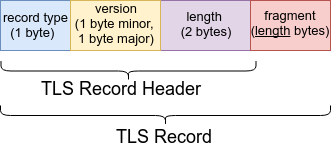
\includegraphics[width=1.0\textwidth]{img/record-header-3.png} % first figure itself
        \caption{\label{fig:tls-record-header} TLS Record header}
    \end{minipage}\hfill
    \begin{minipage}{0.47\textwidth}
        \centering
        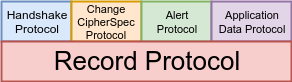
\includegraphics[width=1.0\textwidth]{img/tls-sub-protocols-3.png} % second figure itself
        \caption{\label{fig:tls-subprotocols} TLS (Sub)protocols and Layers}
    \end{minipage}
\end{figure}

\paragraph{TLS Connections and Sessions}

it is important to distinguish between a \textbf{TLS session} and a \textbf{TLS connection}.
\begin{itemize}
  \item \textbf{TLS sesion} - assosciation between two communicationg peers that is
  created by the \textbf{TLS Handshake Protocol}, wich defines a set of negotiated paramters
  (cyrptographic and others, depending on the \gls{tls} version, such as
  the compression algorithm) that are used by the \textbf{TLS connections associated
  with that session}. A single \textbf{TLS session} can be shared among multiple
  \textbf{TLS connections} and its main purpuse is to avoid the expensive negotiation
  of new parameters for each \textbf{TLS connection}. For example, let us say
  that an \gls{html} page is being downloaded over \gls{https} and that page references some images from that same server, using \gls{https} links. Instead of the web browser negotiating a new \gls{tls} session again, it can re-use the the
  one it has established to download the \gls{html} page in the first place,
  saving time and computational resources. Session resumption can be done using various
  approaches, such as \textbf{session identifiers}, described throughout \codeword{Section 7.4}
  of \codeword{RFC 5246} \cite{RFC5246}, \textbf{session tickets}, defined in
  \codeword{RFC 5077} \cite{RFC5077}.
  \item \textbf{TLS connection} - used to actually transmit the cryptographically
  protected data. For the data to be cryptographically protected, some parameters,
  such as the \codeword{secret keys} used to encrypt and authenticate the transmitted
  data need to be established; this is done when a \textbf{TLS session} is created,
  during the \textbf{TLS Handshake Protocol}.
\end{itemize}

\subsubsection{\gls{tls} Record Processing}
A \gls{tls} record must go through some processing before it can tbe sent over the netwrok.
This processing involves the following steps (\codeword{4} for \gls{tls} $1.2$ and \codeword{3} for \gls{tls} 1.3):

\begin{enumerate}
  \item \textbf{Fragmentation} - the \gls{tls} \codeword{Record Layer} takes arbitrary-length data and \textbf{fragments}
  it into manageable pieces: each one of the resulting fragments is called a \codeword{TLS Plaintext}.
  Client message boundaries are not preserved, which means that multiple messages
  of the same type may be placed into the same fragment or a single message may
  be fragmented across several records.
  \item  \textbf{Compression} (removed in \gls{tls} 1.3) - the \codeword{TLS Record Layer} compresses the
  \codeword{TLSPlaintext} structure according to the negotiated compression method,
  outputting \codeword{TLSCompressed}. Compression is optional. If the negotiated compression
  method is \codeword{null}, \codeword{TLSCompressed} is the same as \codeword{TLSPlaintext}.
  \item \textbf{Cryptographic Protection} - in case of \gls{tls} 1.2, either an
  \gls{aead} cipher or a separate encryption and \gls{mac} functions transform a
  \codeword{TLSCompressed} fragment into a \codeword{TLSCipherText} fragment. In case
  of \gls{tls} 1.3, the \codeword{TLSPlaintext} fragment is transformed into a \codeword{TLSCipherText}
  by applying an \gls{aead} cipher.
  \item Append the \textbf{TLS Record Header} - encapsulate \codeword{TLSCipherText}
  in a \codeword{TLS Record}.
\end{enumerate}

\begin{figure}
  \caption{\label{fig:tls-record-processing}TLS Record Processing}
  \centering
  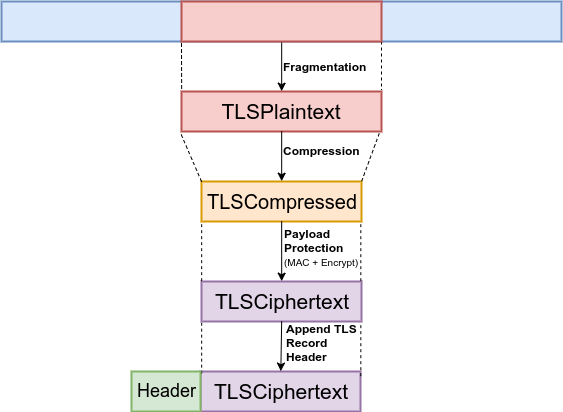
\includegraphics[width=1.0\textwidth]{img/tls-record-processing-3.png}
\end{figure}

The process described above, as well as the structure names are depicted in figure \ref{fig:tls-record-processing}.
Step \codeword{2} is not present in \gls{tls} 1.3. The structure names are exactly as the appear in the \gls{tls} specifications.

\subsubsection{TLS Keying Material}

Secret keys are at the base of most cryptographic operations.
In order for both communicating peers to be able to encrypt and decrypt data
using symmetric cyrpto aglorithms, they need to \textbf{share} the same key
somehow. In \gls{tls}, both, the client and a server derive the \textbf{same set of keys}
independetely, through the exchanged messages in the \gls{tls} Handshake Protocol.

When communicating with one another, the client uses one key to
encrypt the data to be sent to the server and another different key to decrypt the data
that it receives from the server. This means that in order to deal with data
encryption and decryption, both of the communicating entities have two keys:
one to encrypt the outgoing data and one to decrypt the incoming data. Those keys
have different names in \gls{tls} $1.2$ and \gls{tls} 1.3, but they serve the same
basic purpose. In this general description, they will be referred as \codeword{client_write key}
(used by the client to encrypt the data to be sent), \codeword{client_read_key}(used by the client to
decrypt the incoming data from the server), \codeword{server_write_key}(used by the server to encrypt
the data to be sent) and \codeword{server_read_key}(used by the server to decrypt the incoming
data from the client). Note, that the following relationships must hold:
\codeword{client_write_key == server_write_key} and \codeword{client_read_key == server_write_key}.

Besides the secret keys mentioned previously, in \gls{tls} $1.2$ you might also have other ones,
depending on the cipher suite in use, namely the \codeword{client/server_wirite_IV} that
is only generated for implicit nonce techniques used with \gls{aead} ciphers and the
\codeword{client/server_write_MAC_key}, which is the input secret to the \gls{mac}
function; this key is not present when \gls{aead} ciphers are in use.

\subsubsection{TLS 1.2 Keying Material Generation}

The generation of secret keys, used for various cryptographic operations involves the
following steps (in order):

\begin{itemize}
  \item Generate the \textbf{premaster secret}.
  \item From the \textbf{premaster secret} generate the \textbf{master secret}.
  \item From the \textbf{master secret} generate the various secret keys, which
  will be used in the cryptographic operations.
\end{itemize}

In \gls{tls} 1.2, the \gls{tls} \gls{prf} is used to generate the keying material
needed for a connection, which is defined as \codeword{PRF(secret, label, seed) = P_hash(secret, label + seed)}
The \codeword{P_hash(secret, seed)} function is an auxiliary data expansion function
which uses a single cryptographic hash function to expand a \codeword{secret} and a \codeword{seed}
into an arbitrary quantity of output, meaning that you can use to to generate
anywhere from $1$ to an infinite number of bits of output. The \codeword{PRF(secret, label, seed)}
is used to generate as many bits of output as you need. When generating the
master secret, the \codeword{secret} input is the \codeword{premaster secret}.
When generating the key block, from which you will actually obtain final keys
the \codeword{secret} input is the \codeword{master secret}.

The cryptographic hash function used in \codeword{P_hash(secret, label, seed)} is
a hash function implicitly defined by the cipher suite in use. All of the cipher
suites defined in the \gls{tls} $1.2$ base spec use \codeword{SHA-256} and any new
cipher suites must explicitly specify a the same hash function or a stronger one.

\subsubsection{TLS 1.3 Keying Material}

\gls{tls} 1.3's keying material generation is a little more complex, since different
keys are used to encrypt data throughout the Handshake Protocol. This can be
explained by the fact that in \gls{tls} $1.3$ the encryption begins earlier, with
Handshake messages besides the \codeword{Finished} being encrypted,
as well as features such as \textbf{early client data}, also known as \textbf{0-RTT data},
where data comes encrypted in the first flight. As a result of those properties,
you have multiple encryption keys generated and used to encrypt different data
throughout the handshake.

The way the keying material is derived is also different, since the
\gls{prf} construction described above has been replaced. The
new design allows easier analysis by cryptographers due to the improved
key separation properties. In \gls{tls} 1.3, key derivation uses the
\gls{hkdf} function defined in \codeword{RFC 5869}\cite{RFC5869} and its two components,
the \codeword{HKDF-Extract} and \codeword{HKDF-Expand}.

\subsubsection{TLS 1.2 Key Exchange Methods}

The way the \textbf{permaster secret} is generated depends on the key exchange
method used. In fact, this is the only phase of the keying material generation
phase that is variable for a fixed cipher suite (because a cipher suite defines
the \gls{prf} function to be used), the rest remains exactly the same. The derivation
of the \textbf{master secret} from the \textbf{premaster secret}, as well as the
derivation of the bulk encryption keys, \gls{mac} keys and \gls{iv}s from the \textbf{master secret}
that follows \textbf{is not impacted by the key exchange method} in use.

You have quite a few choices when it comes to key exchange methods. Some of them
are defined in the base spec (\codeword{RFC5246} \cite{RFC5246}), while others
in separate \codeword{RFCs} (such as the \gls{ecc} based key exchange, specified
in \codeword{RFC4492} \cite{RFC4492}).

The base spec specifies 4 key exchange methods, one using \gls{rsa} and 3 using
\gls{dh}:

\begin{itemize}
  \item static \gls{rsa} (\codeword{RSA}) [removed in \gls{tls} 1.3] - the client generates the \gls{pms}, encrypts it with the
  server's \gls{pubk} (which it obtained from the server's \codeword{X.509}certificate),
  sending it to the server, which decrypts it using the corresponding \gls{privk}.
  This key exchange method offers authenticity, but does not offer \gls{pfs}.
  \item anonymous \gls{dh} (\codeword{DH_annon}) [removed in \gls{tls} 1.3] - a \gls{dh} key exchange is
  performed and an \textbf{ephemeral} key is generated, but the exchanged \gls{dh}
  parameters are \textbf{not authenticated}, making the resulting key exchange
  vulnerable to \gls{mitm} attacks. \gls{tls} $1.2$ spec states that cipher suites
  using \codeword{DH_annon} \textbf{must not} be used, unless the application
  layer explicitly requests so. This key exchange offers \gls{pfs}, but no
  authenticity.
  \item fixed/static \gls{dh} (\codeword{DH}) [removed in \gls{tls} 1.3] - the server's/client's public \gls{dh} parameter
  is embedded in its certificate. This key exchange method offers authenticity,
  but does not offer \gls{pfs}.
  \item epehemeral \gls{dh} (\codeword{DHE}) - each run of the protocol, uses
  different pubic \gls{dh} parameters, which are generated dynamically. This results
  in a different, epehemeral key being generated every time. The public parameters
  are then digitally signed in some way, usually using the sender's private
  \gls{rsa} (\codeword(DHE_RSA)) or \gls{dsa} (\codeword{DHE_DSS}) key. This key
  exchange offers both authenticity and \gls{pfs}.
\end{itemize}

When either of the \gls{dh} variants is used, the value resulting from the exchange is used
as the \gls{pms} (without the leading \codeword{0}'s). Usually, only the server's
authenticity is desired, but client's can also be achieved if it provides the
server its certificate. Whenever the server is authenticated, the server is secure
against \gls{mitm} attacks. Table \ref{kemsp} summarizes the security properties
offered by each key exchange method.

\begin{table}[]
\centering
\caption{Key exchange methods and security properties}
\label{kemsp}
\begin{tabular}{|l|c|l|}
\hline
\textbf{Key Exch Meth} & \multicolumn{1}{l|}{Authentication} & PFS                    \\ \hline
RSA                          & X                                   &                        \\ \hline
DH\_anon                     & \multicolumn{1}{l|}{}               & \multicolumn{1}{c|}{X} \\ \hline
DH                           & X                                   &                        \\ \hline
DHE                          & X                                   & \multicolumn{1}{c|}{X} \\ \hline
\end{tabular}
\end{table}

Note that in \gls{tls} 1.3, all of static \gls{rsa} and \gls{dh} cipher suites
have been removed: all of the \gls{pubk} exchange methods now provide \gls{pfs}.
Even though, anonymous \gls{dh} has also been removed from \gls{tls} 1.3, you can
still have unauthenticated connections by either using \textbf{raw public keys} \cite{RFC7250}
or by not verifying the certificate chain and any of it is contents.

The \gls{ecc}-based key exchange (\gls{ecdh} and \gls{ecdhe}) and authentication (\gls{ecdsa})
algorithms are defined in \codeword{RFC4292} \cite{RFC4292}, which is also referenced
in \codeword{RFC5246} \cite{RFC4256}. The document introduces five new
\gls{ecc}-based key exchange algorithms, all of which use \gls{ecc} to compute
the \textbf{premaster secret}, differing only in whether the negotiated
keys are epehemeral (\gls{ecdh}) or long-term (\gls{ecdhe}), as well as the mechanism (if any) used to
authenticate them. Three new \gls{ecdsa} \textbf{client authentication} mechanisms are also defined,
differing in the algorithms that the certificate must be signed with, as well
as the key exchange algorithms that they can be used with.
Those features are negotiated through the \gls{tls} Extension Mechanism.

\subsubsection{TLS 1.2 Handshake Protocol}


\begin{figure}
\centering
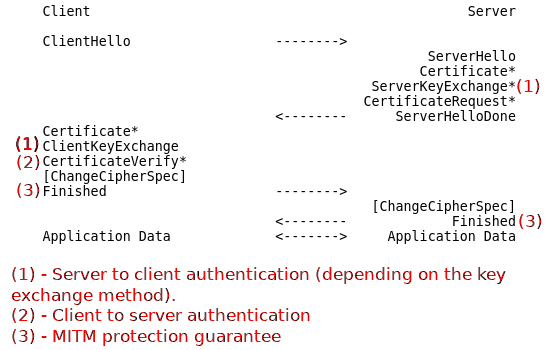
\includegraphics[width=0.9\textwidth]{img/tls-12-full-handshake2.png}
\caption{\label{fig:tls-12-handshake} \gls{tls} $1.2$ message flow for a full handshake}
\end{figure}


In this phase the client and the server agree on which version of the \gls{tls}
protocol to use, authenticate one to another and negotiate items like
the cipher suites and the compression method to use. Figure \ref{fig:tls-12-handshake} shows the message flow for the
full \gls{tls} $1.2$ handshake. Note that \codeword{*} indicates situation-dependent
messages that are not always sent, while \codeword{ChangeCiperSpec} is a separate
protocol, rather than a message type.

As already mentioned before, every \gls{tls} Handshake message is encapsulated within
a \gls{tls} Record. The actual Handshake message is contained within the
\codeword{fragment} of the \gls{tls} Record. The Record type for a Handshake
message is \codeword{0x16}. The Handshake message has the following structure:
a 1-byte \codeword{msg_type} field (specifies the Handshake message type),
a 2-byte \codeword{length} field (specifies the length of the \codeword{body})
and a \codeword{body} field, which contains a structure depending on the
\codeword{msh_type} (similar to \codeword{fragment} field in a \gls{tls} Record).

Now, a typical handshake message flow will be described, with only the most important fields of each message mentioned.

The connections begins with the client sending a \codeword{ClientHello}, containing
.\codeword{random}, \codeword{cipher_suites} and \codeword{compresison_methods},
among other fields.
\codeword{cipher_suites} contains a \textbf{list} of cipher suites and \codeword{compression_methods}
contains a list of compression methods (\codeword{compression_methods}) that the
client supports, ordered by preference, with the most preferred one appearing first.
The \gls{tls} Record contains a \codeword{2-byte} \codeword{version} field which
indicates the highest version supported by the client.

The server responds to the \codeword{ClientHello} with a \codeword{ServeHello}
message, which is similar in its contents, except that instead of containing
a list of supported features, it contains a single item containing the one that it chose,
\textit{i.e.}, the server responds with the chosen \codeword{cipher_suite} and
\codeword{compression_method} (note the \textbf{singular} form) that it chose from the
corresponding list sent by the client. Just like in the client's case, a \codeword{random}
is also present. The \codeword{version} field in the \gls{tls} Record indicates
the \gls{tls} version chosen by the server and it is the one that is gonna be
used for that connection.

\gls{tls} requires cryptographically secure pseudorandom values to be generated
by both of the parties independetely. Those random number (or nonces) are essential for freshness
(protection against replay attacks; we do need both randoms, otherwise the messages could
be replayed) and session uniqueness, since both of
the random values are inputs to the \textbf{master secret} generation, meaning
that a new keying material is generated with every session. If the output of the pseudorandom numbers
can be predicted by the attacker, he can predict the keying material, as described
in "A Systematic Analysis of the Juniper Dual EC Incident"\cite{DualECJu15:online}.
The \codeword{32-byte} random value is composed by concatenating the \codeword{4-byte}
GMT UNIX time with \codeword{28} cryptographically random bytes. Note that in \gls{tls} 1.3
the random number structure has the same length, but is generated in a different manner:
the client's \codeword{32 bytes} are all random, while the server's last \codeword{8 bytes}
are fixed when negotiating \gls{tls} $1.2$ or 1.3.

Next, the server sends a \codeword{Certificate} message, which contains a list
of \gls{pubk} certificates (a certificate chain): the server's certificate,
every intermediate certificate and the root certificate. The certificate's contents
will depend on the negotiated cipher suite and extensions.
The same message type occurs later in the handshake if the server asks the client for certificate with the
\codeword{CertificateRequest} message. Note, that in a typical scenario, the
server will seldom request client authentication.

The \codeword{ServerKeyExchange} message follows, containing additional information
needed by the client to compute the \codeword{premaster secret}. This message
is only sent in some key exchange methods, namely \codeword{DHE_DSS}, \codeword{DHE_RSA}
and \codeword{DH_anon}. For non-anonymous key exchanges, this is the message that authenticates the server to the client,
since the server sends a digital signature over the client and server randoms
and the server's key exchange parameters. Note that this is not the only place where the
server can authenticate itself to the client. For example, if \codeword{RSA} key
exchange is used, the server authentication is done indirectly when the client
sends the premaster secret encrypted with the public RSA key provided in the
server certificate: only the server knows the corresponding private key, so if
both of the sides generate the same keying material, then the server must be who
he claims to. In \gls{tls} $1.3$ this message is non existent and a similar
functionality is taken by the \codeword{key_exchange} extension.

The \codeword{ServerHelloDone} is sent to indicate the end of \codeword{ServerHello}
and associated messages. Upon the receipt of this message, the client should check
that the server provided a valid certificate. This message is not present in \gls{tls} 1.3.

With the \codeword{ClientKeyExchange} message the \codeword{premaster} secret is
set, either by direct transmission of the secret generated by the client
and encrypted with the server's public RSA key (thus, authenticating the server to the client)
or by the transmission of \gls{dh} parameters that will allow each side to generate
the same \codeword{premaster} secret independently.

The \codeword{CertificateVerify} message is sent by the client to verify its
certificate, if it has signing capability (\textit{i.e.} all certificates except for the ones
containing fixed \gls{dh} parameters).

The \codeword{ChangeCipherSpec} is its own protocol, rather than a type of handshake
message. it is sent by both parties to notify the reciever that subsequent records
will be protected under the newly negotiated \codeword{CipherSpec} and keys.

The \codeword{Finished} message is an essential part of the protocol. it is the first
message protected with the newly negotiated algorithms, keys and secrets. Only after
both parties have sent and verified the contents of this message is when they can
be sure that the Handshake has not been tampered with by a \gls{mitm} and begin to
receive and send application data. Essentially, this message contains keyed hash
with the master secret over the hash of all the data from all of the
handshake messages not including any \codeword{HelloRequest} messages and up to, but
not including, this message. The other party must perform the same computation on its
side and make sure that the result is identical to the contents of the other party's
\codeword{Finished} message. If at some point a \gls{mitm} has tampered with the
handshake, the result will be a mismatch in computed and received contents of the
\codeword{Finished} message.

At any time after a session has been negotiated, the server may send a \codeword{HelloRequest}
message, to which the client should respond with a \codeword{ClientHello}, thus
beginning the negotiation process anew.

At an point in the handshake, the Alert protocol may be used by any of the peers
to signal any problems or even abort the process by using an appropriate message type.

Besides the full handshake, the \gls{tls} $1.2$ specification also specifies an
abbreviated handshake mechanism, which can be used to either resume a previous session
or duplicate one, instead of negotiating new security parameters (for example, this is useful
in the context of multiple \codeword{HTTPS} requests for various resources, when loading
a typical website). The advantage of this mechanism is that the handshake is reduced
to \codeword{1 RTT}, instead of the usual \codeword{2 RTT} as it is the case in
the full handshake. In order to do the abbreviated handshake,
the client and the server must have established a session previously, by performing
the full handshake. To do this, the clients sends a session ID of the session it wants to
resume in its \codeword{ClientHello} and its up to the server to decide if he
wants to resume that session, by responding with a \codeword{ServerHello} containing
that same session ID value, or if it wants to establish a new session by
sending a session ID with a different value. The keying material, such as the bulk
data symmetric encryption keys and the \gls{mac} keys are formed by hashing the new client
and server random values with the master secret, which means
that provided that the master secret has not been compromised and that the secure
hash operations are secure, the new connection will be secure and independent
from previous connections. The \gls{tls} $1.2$ spec, suggests and upper limit
of $24$ hours for session ID lifetimes, since an attacker who obtains the master secret
will be able to impersonate the compromised party until the corresponding session
ID is retired. Note that this mechanism requires state to be maintained in both peers.

\subsubsection{TLS Extensions}

\gls{tls} extensions were originally defined in \codeword{RFC 4366}\cite{RFC4366}
and later merged into the \gls{tls} $1.2$ base spec. Each extension consists of an
extension type, which identifies the particular extension type and extension data,
which contains information specific to a particular extension.

The extension mechanism may be used by \gls{tls} clients and servers; it is backwards
compatible, which means that the communication is possible between \gls{tls} a
client that supports a particular extension and a server that does not support it,
and vice versa. A client may request the use of extensions by sending an extended \codeword{ClientHello}
message, which is just a "normal" \codeword{ClientHello} with an additional
block of data that contains a list of extensions. The backwards compatibility is achieved based on the \gls{tls}
requirement that the servers are not "extensions-aware" ignore the data
added to the \codeword{ClientHello}s that they do not understand (section \codeword{7.4.1.2} of \codeword{RFC 2246}\cite{RFC2246}),
meaning that even older servers that do not support extensions, namely the ones with
version of \gls{tls} prior to $1.2$ will not "break".

The presence of extensions can be determined by checking if there are bytes
following the \codeword{compression_methods} field in the \codeword{ClientHello}.
If the server understands an extension, it sends back an extended \codeword{ServerHello},
instead of a regular one. An extended \codeword{ServerHello} is a "normal"
\codeword{ServerHello} with an additional block of data following the
\codeword{compression_method} field that contains a list of extensions.

An extended \codeword{ServerHello} message can only be sent in a response to an
extended \codeword{ClientHello} message. This prevents the possibility that an extended
\codeword{ServerHello} message could "break" older \gls{tls} clients that do not
support extensions. An extension type must not appear in the
extended \codeword{ServerHello}, unless the same extension type appeared in the
corresponding extended \codeword{CleintHello}, and if this happens, the clients must abort the handshake.

\subsubsection{TLS 1.3}

Due to limited space, \gls{tls} $1.3$ will not be described in detail. The focus was on \gls{tls} $1.2$ instead, because \gls{tls} $1.3$ is still in draft
mode and $1.2$ is the latest and the recommended to use version.

Despite the protocol name not suggesting it \gls{tls} $1.3$ is
very different from \gls{tls} 1.2, in fact, it should have probably been called
\gls{tls} 2.0 instead. I have studied \gls{tls} $1.3$ in great detail, and as it was  already mentioned,
I have been formally recognized as a \gls{tls} $1.3$ contributor 1.3.
I have also participated in the mailing lists, as part of my work on the architecture of the solution.

Numerous differences of \gls{tls} $1.3$ from $1.2$ have been mentioned throughout the document.
Various changes in \gls{tls} $1.3$ make it more suitable in the context
of \gls{iot}. Some of them have already mentioned previously, and in this section a couple more will be outlined.

The first important difference is that in \gls{tls} $1.3$ extensions are required,
since some of the functionality has been moved into extensions, in order to preserve
backwards-compatibility with the previous versions of the \codeword{ClientHello}s.
In fact, the way a server distinguishes if a client is requesting a \gls{tls} 1.3
is by checking the presence of the \codeword{supported_versions} extension in the
extended \codeword{ClientHello}.

In \gls{tls} $1.3$ more data is encrypted and the encrytion starts earlier. For example,
on the server-side you have a notion of "encrypted extensions". The \codeword{EncryptedExtensions}
message, as the name suggests, contains a list of extensions that are encrypted
under a symmetric key and it contains any extensions that are not needed
to establish the cryptographic context.

In \gls{tls} 1.3, non \gls{aead} ciphersuites are not supported anymore.
Static RSA and \gls{dh} ciphersuites have been removed, meaning that all
public key exchange mechanisms now provide \gls{pfs}. Even though
anonymous \gls{dh} key exchange has been removed, you can still have
unauthenticated connections by either using raw public keys or not verifying the
certificate and any of its contents.

One of the main problems with using \gls{tls} in \gls{iot} is that while \gls{iot}
traffic need to be quick and lightweight, \gls{tls} $1.2$ adds two additional
round trips (\codeword{2 RTT}) to the start of every session. \gls{tls} $1.3$ handshake has less latency,
when compared to \gls{tls} $1.2$ and this is extremely important in the context of \gls{iot}.
The full \gls{tls} $1.3$ handshake is only \codeword{1 RTT}. \gls{tls} $1.3$ even allows
clients to send data on the first flight (known as "early data"), when the clients
and servers share a \gls{psk} (either obtained externally or via a previous handshake).
This means that in \gls{tls} $1.3$ you can have \codeword{0-RTT} data, by essentially
encrypting it with the previously shared \gls{psk}. Session resumption
via identifiers and tickets has been obsoleted in \gls{tls} 1.3, and both methods
have been replaced by a \gls{psk} mode. The \gls{psk} is established on a previous
connection after the handshake is completed and can be presented by the client
on the next visit.

%
\subsection{DLTS}

The design of \gls{dtls} is intentionally very similar to \gls{tls}, in fact, its specification is written
in terms of differences from \gls{tls}. The changes are mostly done on the lower level,
and even extensions that have been defined before \gls{dtls} has even existed can be
used with \gls{dtls}, The latest version of \gls{dtls} is $1.2$ and it is defined
in \codeword{RFC 6347}\cite{RFC6347}. There is a draft of \gls{dtls} 1.3
\cite{I-D.ietf-tls-dtls13} that is currently under active development.

Since \gls{dtls} operates on top of an unreliable transport protocol, such as
UDP, it must explicitly deal with the absence of reliable and ordered assumptions
that are made by \gls{tls}. The main differences from \gls{dtls} $1.2$ to \gls{tls} $1.2$ are:

\begin{itemize}
  \item two new values are added to the record layer: an explicit \codeword{2 byte} sequence
  number and a \codeword{6 byte} epoch fields. The \gls{dtls} \gls{mac} is the same as of \gls{tls},
  however, rather than using the implicit sequence number, the \codeword{8 byte} value
  formed by concatenation of the epoch number and the sequence number is used.

  \item stream ciphers must not be used with \gls{dtls}.

  \item a stateless cookie exchange mechanism has been added to the handshake protocol
  in order to prevent \gls{dos} attacks. To accomplish this, a new handahke
  message, the \codeword{HelloVerifyRequest} has been added. After
  the \codeword{ClientHello}, the server responds with a \codeword{HelloVerifyRequest}
  containing a cookie, which is returned back to the server in another
  \codeword{ClientHello} that follows it, after which the handshake proceeds as in \gls{tls}.
  Although optional for the server, this mechanism highly recommended, and the
  client must be prepared to respond to it.

  \item the handshake message format has been extended to deal wit message reordering,
  fragmentation and loss by addition of three new fields: a message sequence field,
  a fragment offset field and a fragment length field.
\end{itemize}

\section{Related Work}

Lightweight cryptography is an important topic in the context of \gls{iot}, since
cryptography a fundamental part of security and it is fundamental for it to be
lightweight in order to run on devices with limited memory and processing
capabilities. A lot of work in \gls{iot} incorporates it in one way or another,
so this section will begin with the description of the work done in this area.

Alex \textit{et al}\cite{Stateoft96:online} explore the topic of lightweight symmetric cryptography,
providing a summary of the lightweight symmetric
primitives from the academic community, the government agencies and even proprietary
algorithms which have been either reverse-engineered or leaked. All of those algorithms
are listed in the paper, alongside relevant metrics. The list will not be
included here due to lack of space. The authors also proposed
to split the field into two areas: ultra-lightweight and \gls{iot} cryptography.

The authors systematized the knowledge in the area of lightweight cryptography
in order to define "lightweightness" more precisely. They observed that the design
of lightweight cryptography algorithms vary greatly, the only unifying thread
between them being the low computing power of the devices they are designed to run on.

The most frequently optimized metrics are the memory consumption, the implementation size
and the speed or the throughput of the primitive. The specifics depend on whether
the hardware or the software implementations of the primitives are considered.

If the primitive is implemented in hardware, the memory consumption and the implementation
size are lumped together into its gate area, which is measured in Gate Equivalents (GE),
a metric quantifying how physically large a circuit implementing primitive is.
The throughout is measured in bytes/sec and it corresponds to the amount of plaintext
processed per time unit. If a primitive is implemented in software (typically for
use in micro-controllers), the relevant metrics are the RAM consumption, the code
size and the throughput of the primitive, measured in bytes per CPU cycle.

To accommodate the limitations of constrained devices, most lightweight algorithms
are designed to use smaller internal states with smaller key sizes. After analysis,
the authors concluded that even though at least \codeword{128 bit} block and
key sizes were required from the AES candidates, most of the lightweight
block ciphers use only \codeword{64-bit} blocks, which leads to a smaller memory
footprint in both, software and hardware, while also making the algorithm better suited
for processing smaller messages.

Even though though algorithms can be optimized in implementation: whether it is
a software or a hardware, dedicated lightweight algorithms are still needed.
This comes down mainly to two factors: there are limitations to the the extent of
the optimizations that you can make and the hardware-accelerated encryption is
frequently vulnerable to various \gls{sca}s (such as the attack done on the
Phillips light bulbs \cite{cryptoeprint:2016:1047}, where the authors were able to
recover a secret key used to authenticate updates, via an \gls{sca}).

It is more difficult to implement a lightweight hash function than a lightweight
block cipher, since standard hash functions need large amounts
of memory to store both: their internal states, for example, \codeword{1600 bits} in case of SHA-3
and the block they are operating on, for example, \codeword{512 bits} in the case of SHA-2.
The required internal state is acceptable for a desktop computer, but not for a
constrained device. Taking this into consideration, the most common approach
taken by the designers is to use a sponge construction with a very small bitate.
A sponge function is an algorithm with an internal state that takes as an input
a bit stream of any length and outputs a bit stream of any desired length. Sponge
functions are used to implement many cryptographic primitives, such as cryptographic
hashes. The bitrate decides how fast the plain text is processed and how fast the
final digest is produced. A small bitrate means that the output will take longer
to be produced, which means that a smaller capacity (the security level)
can be used, which minimizes the memory footpirnt at the cost of slower data
processing. A capacity of \codeword{128 bits} and a bitrate of \codeword{8 bits}
are common values for lighweight hash functions.

Another trend in the lightweight algorithms noticed by the authors is the
preference for ARX-based and bitsliced-S-Box based designs, as well as simple
key schedules.

Finally, a separation of the "lightweight algorithms" defintion into two
distinct fields has been proposed:

\begin{itemize}
  \item \textbf{Ultra-Lightweight Crypto} - algorithms running on very cheap
  devices which are \textbf{not connected to the internet}, which are easily replaceable
  and have a limited life-time. Examples: RFID tags, smart cards and remote car keys.
  \item \textbf{IoT Crypto} - algorithms running on a low-power device,
  \textbf{connected to a global network}, such as the internet. Examples: security cameras,
  smart light bulbs and smart watches.
\end{itemize}

Considering the two definitions above, this work focuses on \textbf{IoT Crypto}
devices. A summary of differences between the both categories is summarized in
table \ref{ul-iot}.

\begin{table}[]
\centering
\caption{A summary of the differences between ultra-lightweight and IoT crypto}
\label{ul-iot}
\begin{tabular}{@{}lll@{}}
\toprule
                           & \textbf{Ultra-Lightweight}          & \textbf{IoT}                           \\ \midrule
\textbf{Block Size}        & 64 bits                             & ≥ 128 bits                             \\
\textbf{Security Level}    & ≥ 80 bits                           & ≥ 128 bits                             \\
\textbf{Relevant Attacks}  & low data/time complexity            & same as "regular" crypto               \\
\textbf{Intended Platform} & dedicated circuit (ASIC, RFID...)   & micro-controllers, low-end CPUs        \\
\textbf{SCA Resilience}    & important                           & important                              \\
\textbf{Functionality}     & one per device, e.g. authentication & encryption, authentication, hashing... \\
\textbf{Connection}        & temporary, only to a given hub      & permanent, to a global network         \\ \bottomrule
\end{tabular}
\end{table}

While there is a high demand lightweight \gls{pubk} primitives, the required
resources for them are much higher than for symmetric key ones. As the
\textit{Lightweight Cryptography for the Internet of Things}\cite{b5b8db9716:online} paper
by \textit{Sony Corporation} concluded, there are no promising primitives
that have enough lightweight and security properties, comparing to the
conventional ones, such as RSA and \gls{ecc}. Further research on this topic lead to the same conclusion.

Lightweight cryptography is an important part of my work and there are papers detailing
various algorithms. While an important topic for the final solution, it was covered in sufficient detail, by purposefully describing recent works that
provide an overview of the different areas, rather than focusing on specific
implementations, since the length of this section is limited. The remaining text
in this section will be used to describe work done on the (D)\gls{tls} protocol in the
context of \gls{iot}.

For the reasons above, the main key exchange mechanism used in IoT
are \gls{psk}s. S3K\cite{S3KScala62:online} proposes a key management architecture for resource-constrained devices,
which allows devices that have no previous, direct security relation to use
(D)\gls{tls} using one of two approaches: shared symmetric keys or raw public keys.
The resource-constrained device is a server that offers one or more resources,
such as temperature readings. The idea in both approaches is to introduce a third-party
\codeword{trust anchor (TA)} that both, the client and the server use to establish
trust relationships between them.

The first approach is similar to Kerberos\cite{RFC4120}, without requiring any
changes to the original protocol. A client can request a \gls{psk} \codeword{Kc} from the \codeword{TA},
which will generate it and send it back to the client via a secure channel, alongside
a \codeword{psk_identity} which has the same meaning and is used in the same way
as defined in \codeword{RFC 4279}\cite{RFC4279}. When connecting to the server,
the client will then send the \codeword{psk_identity} that it received in the
the (D)TLS handshake and the server will derive the \codeword{Kc}, using the
\codeword{P_hash()} function defined in \cite{RFC5246}.

The second approach consists in the requesting an APK (the authors never defined
what this acronym stands for, but my assumption is that they mean "Authorization Public Key")
from the TA. In his request,
the client includes his \gls{rpk}, which is used for authorization. The TA
creates an authorizaton certificate, protects it with a MAC and sends it
to the client alongside the server's \gls{pubk}.
The client then sends this APK (instead of the \gls{rpk})
when connecting to the server, which verifies the APK (to authorize the client)
and proceeds with the handshake in the \gls{rpk} mode, as defined in \cite{RFC4279}.
To achieve this, a new certificate structure is defined, alongside a new \codeword{certificate_type}.
The new certificate strucure is just the RFC7250 \cite{RFC7250} structure, with an
additonal MAC.

The has function used for key derivation is SHA256. The authors evaluated the
performance of their solution with and without SHA2 hardware acceleration and
concluded that while it had significant impact on key derivation, it had little
impact on the total handshake time (\codeword{711.11 ms} instead of \codeword{775.05 ms}), since most of the time was spent in sending
data over the network and other parts of the handshake, the longest one being
the \codeword{ChangeCiperSpec} message which required the longest processing time
of \codeword{17.79ms}.

6LoWPAN\cite{RFC4944} is a protocol that allows devices with limited processing
ability and power to transmit information wirelessly using the \codeword{IPv6}
protocol. The protocol defines IP Header Compression(IPHC) for the IP header and
Next Header Compression (NHC) for the IP extension headers and the UDP header in \cite{RFC6282}.
The compression relies on the shared context between the communicating peers.

\cite{6LoWPANC53:online} uses this same idea, but with the goal of compressing DTLS headers.
6LoWPAN does not provide ways to compress the UDP payload and layers above, there
is however, a proposed standard\cite{RFC7400} for generic header compression
for 6LoWPANs that can be used to compress the UDP payload. The authors propose
a way to compress DTLS headers and messages using this mechanism.

The paper \cite{6LoWPANC53:online} defines how the \gls{dtls} Record header, the \gls{dtls} Handshake header,
the ClientHello and the ServerHello messages can be compressed, but notes that
the same compression techniques can be used to compress the remaining Handshake
messages. They explore two cases for the header compression: compressing both,
the Record header and the Handshake header and compressing the Record header only,
which is useful after the handshake has completed and the fragment field of the
Record layer contains application data, instead of a handshake message.

\begin{figure}
    \centering
    \begin{minipage}{0.5\textwidth}
        \centering
        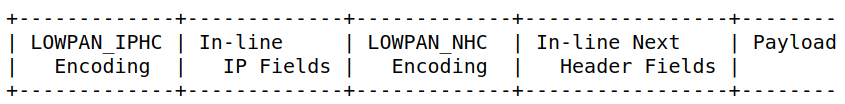
\includegraphics[width=1.0\textwidth]{img/6lowpan-header.png} % first figure itself
        \caption{\label{fig:6lowpan-header} IPv6 Next Header Compression}
    \end{minipage}\hfill
    \begin{minipage}{0.5\textwidth}
        \centering
        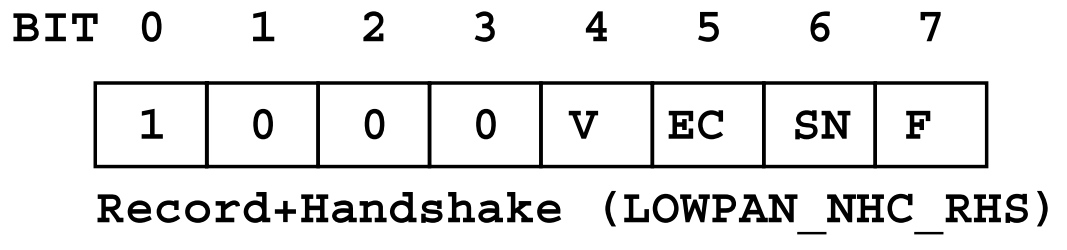
\includegraphics[width=1.0\textwidth]{img/6lowpan-ghc-rhs.png} % second figure itself
        \caption{\label{fig:6lowpan-ghc-rhs} LOWPAN\_NHC\_RHS structure}
    \end{minipage}
\end{figure}


All of the cases follow the same basic idea, for this reason only one of them will be exemplified. Each \gls{dtls} fragment is carried over in the UDP payload. In this case,
the UDP payload carries a header-like payload (the DTLS record header).
Figure \ref{fig:6lowpan-header} shows the way IPv6 next header compression is done.
The authors use the same value for the \codeword{LOWPAN_NHC Encoding} field (defined in \cite{RFC6282})
as in \codeword{RFC7400} and define the format of the \codeword{In-line Next Header Fields}
(defined in \cite{RFC6282}), which is the compressed DTLS content. The \codeword{LOWPAN_IPHC Encoding}
and \codeword{In-Line IP Fields} fields are used in the IPv6 header compression
and are not in the scope of the paper.

The case where both, the Record and the Handshake headers are compressed
will be exemplified.
In this case \codeword{LOWPAN_NHC Encoding} will contain the \codeword{LOWPAN_NHC_RHS}
structure (depicted in figure \ref{fig:6lowpan-ghc-rhs}), which is the compressed form of the Record and Handshake headers. The
parts that are not compressed will be contained in the \codeword{Payload} part.
The first four bits represent the ID field and in this case they are fixed to \codeword{1000},
so that the decompressor knows what is being compressed (\textit{i.e} how to interpret
the structure that follows the ID bits). If the \codeword{F} field of the \codeword{LOWPAN_NHC_RHS} structure contains the
bit \codeword{0}, it means that the handshake message is not fragmented, so
the \codeword{fragment_offset} and \codeword{fragment_length} fields are
elided from the Handshake header (common case when a handshake message is not bigger than
the maximum header size), meaning that they are not going to be sent at
all (\textit{i.e.} they are not going to be present in the \codeword{Payload} part).
If the \codeword{F} bit has the value \codeword{1}, the \codeword{fragment_offset}
and \codeword{fragment_length} fields are carried inline (\textit{i.e.} they are
present in the \codeword{Payload} part). The remaining two fields define similar
behavior for other header fields (some of them assume that some default value is present, when a field is elided).
The \codeword{length} field in the Record and Handshake headers are always elided,
since they can be inferred from the lower layers.

The evaluation showed that the compression can save a significant number of bits:
the Record header, that is included in all messages can be compressed by \codeword{64 bits}
(\textit{i.e.} by \codeword{62\%}).

There is also a proposal for TCP header compression for 6LoWPAN\cite{I-D.aayadi-6lowpan-tcphc},
which if adopted, in many cases can compress the mandatory \codeword{20 bytes} TCP header
into \codeword{6 bytes}. This means that the same ideas can be applied to TCP and
TLS as well.

Later, in 2013, Raza \textit{et al.} proposed a security scheme called Lithe\cite{LitheLig40:online},
which is a lightweight security solution for \gls{coap} that uses the same DTLS header
compression technique as in \cite{6LoWPANC53:online} with the goal of implementing
it as a security support for \gls{coap}.\gls{coap}\cite{RFC7959} is a specialized
RESTful Internet Application Protocol for constrained devices. it is designed to easily
translate to HTTP, in order to simplify its integration with the web,
while also meeting requirements such as multicast support and low overhead.
\gls{coap} is like "HTTP for constrained devices".
\gls{coap} can run on most devices that support UDP or a UDP-like protocol.
\gls{coap} mandates the use of \gls{dtls} as the underlying security protocol for
authenticated and confidential communication. There is also a specification \gls{coap}
running on top of TCP, which uses \gls{tls} as its underlying security protocol
currently being proposed \cite{I-D.ietf-core-coap-tcp-tls},
with active work being done in this area.


The authors evaluated their system in a simulated environment in Contiki OS and
they obtained significant gains in terms of packet size (similiar numbers to the
ones obsever in \cite{6LoWPANC53:online}), energy consumption (in average \codeword{15\%} less
energy is used to transmitting and receive compressed packets), processing time
(the compression and decompression time of DTLS headers is almost negligible)
and network-wide response times(up to \codeword{50\%} smaller RTT). The
gains in the mentioned measures are the largest when the compression avoids
fragmentation (in the paper, for payload size of \codeword{48 bytes}).

Angelo \textit{et al} \cite{Security5:online} proposed to integrate the \gls{dtls} protocol
inside the \gls{coap}, while also exploiting \gls{ecc} optimizations and minimizing
ROM occupancy. They have implemented their solution on an off-the-shelf mote platform
and evaluated its performance. \gls{dtls} was designed to protect web application communication, as a result,
it has a big overhead in \gls{iot} scenarios. Besides that, it runs over UDP,
so additional mechanisms are needed to provide the reliability and ordering
guarantee. With this in mind, the authors wanted to design a version of \gls{dtls}
that is both: minimizes the code size and the number of exchanged messages, resulting
in an optimized Handshake protocol.

In order to minimize the code size occupied by the \gls{dtls} implementation, they
decided to delegate the tasks of \textbf{reliability} and \textbf{fragmentation} to
\gls{coap}. This means that the code responsible for those functionalities,
can be removed altogether from the \gls{dtls} implementation, thus reducing ROM
occupancy. This part of their work was based on an informational RFC draft\cite{I-D.keoh-dtls-profile-iot}, in which the
authors profiled \gls{dtls} for \gls{coap}-based \gls{iot} applications and proposed
the use of a RESTful \gls{dtls} Handshake which relies on \gls{coap} block-wise
transfer to address the fragmentation issue.

To achieve this they  proposed the use of a RESTful \gls{dtls} connection as a \gls{coap} resource,
which is created when a new secure session is requested.
The authors exploit the the \gls{coap}s capability to provide connection-oriented
communication offered by its message layer. In particular, each \codeword{Confirmable}
\gls{coap} message requires an \codeword{Acknowledgement} message (page 8 of \cite{RFC7252}),
which acknowledges that a specific \codeword{Confirmable} message has arrived, thus
providing reliable retransmission.

Instead of leaving the fragmentation function to \gls{dtls}, it was
delegated to the block-wise transfer feature of \gls{coap}\cite{RFC7959}, which was developed
to support transmission of large payloads. This approach has two advantages: first, the code in the \gls{dtls}
layer responsible for this function can be removed, thus reducing ROM occupancy
and second, the fragmentation/reassembly process burdens the lower Layers
with state that is better managed in the application layer.

The authors also optimized the implementation of basic operations on which
many security protocols, such as \gls{ecdh} and \gls{ecdsa} rely upon. The first
optimization had to do with modular arithmetic on large integers. A set of optimized
assembly routines based on \cite{Comparin25:Online} allow the improved use of
registers, reducing the number of memory operations needed to perform
operations such as multiplications and square roots on devices with \codeword{8-bit}
registers.

Scalar multiplication is often the most expensive operation in \gls{ec} based
cryptography, therefore optimizing it is of high interest. The authors used a
technique called \textit{IBPV} described in \cite{LowcostS87:online}, which is based on precumputation
of a set of Discrete Log pairs. The mathematical details have been purposefully omitted,
since they are not relevant for this description. The \textit{IBPV} technique was used
to improve the performance of the \gls{ecdsa} signature and was also extended to the
\gls{ecdh} protocol. In order to reduce the time it takes to do the \gls{ecdsa}
signature verification, the \textit{Shamir trick} was used, which allows
to perform the sum of two scalar multiplications (frequent operation in \gls{ec} cryptography)
faster than performing two independent scalar multiplications.

The results showed that the \gls{ecc} optimizations
outperform the scalar multiplication in the state of the art class 1 device platforms,
while also improving the the network lifetime by a factor of up to $6.5$ with
respect to a standard, non-optimized implementation. Leaving reliability and
fragmentation tasks to \gls{coap}, reduces the \gls{dtls} implementation code size
by approximately $23\%$.

\codeword{RFC 7925}\cite{RFC7925} describes a \gls{tls} and \gls{dtls} 1.2
profile for \gls{iot} devices that offers communication security services
for \gls{iot} applications and is reasonably implementable on many constrained devices.
In this context, "profile" means available configuration options (ex: which
cipher suites to use) and protocol extensions that are best suited for \gls{iot} devices.
The document is rather lengthy, only its fundamental parts will be summarized. Some \gls{rfc}s that are relevant to this will also be described.

The RFC explores both cases constrained clients and constrained servers, specifying
a profile for each one and describing the main challenges faced in each scenario.
The profile specifications for constrained clients and servers are very similar.
Code reuse in order to minimize the implementation size is recommended. For example, an \gls{iot} device
using a network access solution based on \gls{tls}, such as EAP-TLS\cite{rfc5216}
can reuse most parts of the code for (D)TLS at the application layer.

For the credential types the profile considers 3 cases:

\begin{itemize}
  \item \gls{psk} - authentication based on \gls{psk}s is described in
  \codeword{RFC 4249}\cite{RFC4279}. When using \gls{psk}s, the client indicates which
  key it uses by including a \gls{psk} identity in its ClientKeyExchange message.
  A server can have different \gls{psk} identities shared with different clients.
  An identity can have any size, up to a maximum of \codeword{128 bytes}.
  The profile recommends the use of shorter \gls{psk} identities and specifies
  \codeword{TLS_PSK_WITH_AES_128_CCM_8} as the only mandatory-to-implement
  ciphersuite to be used with \gls{psk}s, just like \gls{coap} does. \gls{pfs} is
  a property that preserves the confidentiality of past interactions even if the
  long-term secret is compromised. If a \gls{pfs} ciphersuite is used, ephemeral
  \gls{dh} keys should not be reused over multiple protocol exchanges.

  \item \gls{rpk} - the use of \gls{rpk}s in (D)TLS is described in \codeword{RFC 7250}\cite{RFC7250}.
  With \gls{rpk}s, only a subset of the information is found in typical certificates
  is used: namely the \codeword{SubjectPublicKeyInfo} structure, which contains
  the necessary parameters to describe the public key (the algorithm identifier
  and the public key itself). Other PKIX certificate\cite{RFCabc} parameters are
  omitted, making the resulted \gls{rpk} smaller in size, when compared to the
  original certificate and the code to process the keys simpler. In order for the
  peers to negotiate the \gls{rpk} use, two new extensions have been defined:
  one for the client to list the certificate types that it supports (sorted by order of preference) and one for
  the indicate which one it chose. To further reduce the size of the implementation, the \codeword{RFC 7250}
  recommends the use of the \gls{tls} Cached Information extension\cite{RFC7924}, which
  enables the \gls{tls} peers to exchange just the fingerprint (a shorter sequence of bytes
  used to identify a \gls{pubk}) of the \gls{pubk}. The only mandatory-to-implement
  ciphersuite to be used with \gls{rpk}s is \codeword{TLS_ECDHE_ECDSA_WITH_AES_128_CCM_8},
  just like with \gls{coap}. Note that the ciphersuite makes the use of \gls{aead}.

  \item certificate - conventional certificates can also be used. The support
  for the Cached Information extension\cite{RFC7924} and the \codeword{TLS_ECDHE_ECDSA_WITH_AES_128_CCM_8}
  ciphersuite is required. The profile restricts the use of named curves to
  the ones defined in \cite{RFC4492}. For certificate revocation, neither the
  \gls{ocsp}\cite{RFC6960}, nor the \gls{crl}\cite{RFCabc} mechanisms are used, instead this task is delegated to
  the software update functionality. The Cached Information extension does not
  provide any help with caching client certificates. For this reason, in cases
  where client-side certificates are used and the server is not constrained,
  the support for client certificate URLs is required. The client certificates URL
  extension\cite{RFC4366} allows the clients to point the server to a URL from
  which it can obtain its certificate, which allows constrained clients to
  save memory and amount of transmitted data. The Trusted CA Indication\cite{RFC6066}
  extension allows the clients to indicate which trust anchors they support, which is useful
  for constrained clients that due to memory limitation posses only a small number
  of \gls{ca} root keys, since it can avoid repeated handshake failures. If the clients interacts with
  dynamically discovered set of (D)TLS servers, the use of this extension is recommended,
  if that set is fixed, it is not recommended.

\end{itemize}

The signature algorithms extension\cite{RFC5246} allows the client to indicate
to the server which signature/hash pairs it supports to be used in digital signatures.
The client must send this extension to indicate the use of \codeword{SHA-256},
otherwise the defaults defined in \cite{RFC5246} are used. This extension is not
applicable when the \gls{psk}-based ciphersuites are used.

The profile mandates that constrained clients must implement the session
resumption to improve the performance of the handshake since this will lead to
less exchanged messages, lower computational overhead, since only symmetric cyrptography
is used, and it requires less bandwidth. In case the server is constrained, but
the client is not, the client must implement the Session Resumption Without
Server-Side State mechanism\cite{RFC5077}, which is achieved through the
use of tickets. The server encapsulates the state into a ticket and forwards it to
the client, which can subsequently resume the session by sending back that ticket.
If both, the client and the server are constrained, both of them should implement
\codeword{RFC 5077}\cite{RFC5077}.

The use of compression is not recommended for two reasons. First, \codeword{RFC7525}\cite{RFC7525}
recommends disabling (D)TLS level compression, due to attacks such as \codeword{CRIME}\cite{Microsof72:online}.
\codeword{RFC7525} provides recommendations for improving the security of deployed services
that use \gls{tls} and \gls{dtls} and was published as a response to the various
attacks on (D)TLS that have emerged over the years. Second, for \gls{iot} applications,
the (D)\gls{tls} compression is not needed, since application-layer protocols are hightly
optimized and compression at the (D)TLS layer increases the implementation's size and complexity.

\codeword{RFC6520} defines a heartbeat mechanism to test whether the other peer
is still alive. The implementation of this extension is recommended for server
initiated messages. Note that since the messages to the client will most likely
get blocked by the middleboxes, the initial connection set up is initiated by the
client and then kept alive by the server.

Many of the usual sources of entropy, such as the timing of keystrokes and the
mouse movements will not be available on many \gls{iot} devices, which means that
either alternative ones need to be found or dedicated hardware must be added.
\gls{iot} devices using (D)\gls{tls} must find ways to offer to generate quality
random numbers, the guidelines and requirements for which can be found in \codeword{RFC4086}\cite{rfc4086},
since they play an essential role in the overall security of the protocol.

Implementations compliant with this profile must use \gls{aead} ciphers, this means
that encryption and \gls{mac} computation are no longer independent steps, which means
that neither encrypt-then-MAC\cite{RFC7366}, nor the truncated MAC\cite{RFC6066} extensions are applicable
to this specification and must not be used.

The \gls{sni} extension\cite{RFC6066} defines a mechanism for a client to
tell a (D)TLS server the name of the server it wants to connect to. This is
crucial in case when multiple websites are hosted under the same IP address.
The implementation of this extension is required, unless the (D)\gls{tls}
client does not interact with a server in a hosting environment.

The maximum fragment length extension\cite{RFC6066} lowers the maximum fragment
length support of the record layer from $2^14$ to $2^9$. This extension allows
the client to indicate the server how much of the incoming data it is able to buffer,
allowing the client implementations to lower their RAM requirements, since it does not
not need to accept packets of large size, such as the 16K packets required by
plain (D)\gls{tls}. For that reason, client implementations must support this
extension.

The Session Hash Extended Master Secret Extension \cite{RFC7627} defines an extension
that binds the master secret to the log of the full handshake, thus preventing
\gls{mitm} attacks, such as the tripple handshake\cite{TripleHa89:online}. Even though the
ciphersuites recommended by the profile are not vulnerable to this attack, the
implementation of this extension is advised. In order to prevent the renegotiation
attack\cite{RFC5746}, the profile requires the \gls{tls} renegotiation feature
to be disabled.

With regards to the key size recommendations, the authors recommend symmetric keys
of at least \codeword{112 bit}, which corresponds to a \codeword{233-bit} \gls{ecc}
key and to a \codeword{2048} \gls{dh} key. Those recommendations are made
conservatively under the assumption that \gls{iot} devices have a long expected
lifetime ($10+$ years) and that those key recommendations refer to the long-term
keys used for device authentication. Keys that are provisioned dynamically
and used for protection of transactional data, such as the ones used in
(D)\gls{tls} ciphersuites, may be shorter, dependent on the sensitivity of
transmitted data.

Even though \gls{tls} defines a single stream cipher: the RC4, its use is no longer
recommended due to cryptographic weaknesses described in \codeword{RFC 7465}\cite{RFC7465}.

The \codeword{RFC 7925}\cite{RFC7925} points out the importance of designing a software
update mechanism into an \gls{iot} system is crucial to ensure that potential vulnerabilities
can be fixed and that the functionality can be enhanced. The software update mechanism
is important to change configuration information, such as trust anchors and
other secret-key related information. Although the profile refers to \codeword{LM2M}\cite{OpenMobi29:online}
as an example of protocol that comes with a suitable software update mechanism,
there has been new work done in this area since the release of this profile.
Namely, there is a document specifying an architecture for a frimware update
mechanism for \gls{iot} devices\cite{I-D.moran-suit-architecture} currently in "Internet-Draft" state.

\section{Solution}

\subsection{Solution Architecture}

Most of the work that has been done has been centered around \gls{dtls},
even though most of the solutions can be applied to both.
Herein we want to explore \gls{tls} optimization more. There is clearly a need for that, specially with \gls{coap} over
TCP and \gls{tls} standard being currently developed. The \gls{coap}\cite{RFC7252} protocol is the HTTP
for constrained devices and the mentioned standard does not explore any \gls{tls}
optimizations, and since any \gls{iot} device using it in the future would benefit
them, this is an important area to explore. None of the related work centered around
(D)\gls{tls} 1.3, mainly this is because the protocol is still in draft stages, major design changes however, should not be expected at this point.

Most of the work done in this area proposes a solution that is tied to a
specific protocol, such as \gls{coap}, or requires an introduction of a third-party
entity, such as the trust anchor in the case of S3K\cite{S3KScala62:online} or
even both. This two main issues: first, if the developer wants to use (D)\gls{tls}
without using any specific protocol for which the solution was tuned for (such as \gls{coap}),
he might see himself in some trouble, and second the requirement of a third-party
introduces additional cost and complexity, which will be a big resistance factor>
in adopting that technology. This is specially true for developers who are doing
hobby projects or projects for small businesses, leaving the communications insecure
in the worse case scenario. The goal of this work is to design a solution that can be used out
of the box and is not tailored towards any specific protocol, that is fully backwards
compatible with the original protocol, that can be used with either \gls{tls}
or \gls{dtls} and would work with both versions: (D)\gls{tls} $1.2$ and the upcoming
(D)\gls{tls} 1.3.

In order to achieve the goals described in this document above, the extension
mechanism of \gls{tls} will be heavily relied upon. By using extensions, any deviations from the original protocol an be done, even if they completely change the it. This was confirmed by
one of the \gls{tls} designers, after I asked this question on the official
\gls{ietf} mailing list\cite{ReTLSTLS31:online}, since neither of the four versions of the \gls{tls} protocol
specifications, nor \codeword{RFC 4366} made it clear.

Ideas from \gls{tls} $1.3$, such as \codeword{0-RTT data}, which can be done if peers already share a \gls{psk} would be interesting to implement in the second part of the work.
For example, this can be very useful in the context of the temperature sensor
described in the introduction, where the sensors sends data to a server every
30 seconds. With \codeword{0-RTT data}, it can communicate securely with minimal costs.
The use of symmetric crytpography exclusively, has various additional advantages in the context
of \gls{iot}, which were already mentioned, so there is value in exploring solutions that revolve around
\gls{psk}s and that avoid public key cryptography altogether.

Not all \gls{iot} devices are limited to the point of not being able to use
public key crytpography at all. For some of them, the use of something like raw
public keys, which is considered the first entry point into the area of \gls{pubk}
crytpography, is acceptable, while others are powerful enough to take
advantage of certificates and \gls{pki}, at least up to some point. My solution
would be adaptable to any of those scenarios, depending on the context and the security
requirements, therefore being similar to a framework. For example, some scenarios
might not require integrity, but not privacy. For those, it makes no sense to
pay the energy and time overhead of encryption. Special care in the
selection of cipher suites and key exchange methods needs to be taken, possibly even developing new ones.

(D)\gls{tls} $1.2$ is significantly different from (D)\gls{tls} 1.3
and there has been no work like \codeword{RFC 7924}\cite{RFC7924} done for (D)TLS 1.3
and it would be interesting to explore this. \gls{tls} $1.3$ has many fundamental changes
to the way the handshake is done, bringing many new features, whose ideas can
be incorporated into my proposed solution and even backported to \gls{tls} 1.2.

\subsection{Evaluation}

In order to evaluate how good the result of the work is, both, the original protocol
implementation and the one provided as part of the solution, will be profiled and compared. The relevant profiling metrics are power consumption, RAM usage, storage usage,
CPU cycles used and time taken. The profiling
will be done over various simulated scenarios, which emulate real-life usage,
such as connecting to the server multiple times over a short time period and transfer
small quantity of data, connecting to the server and transferring a large
amount of data all at once, and so on.

Due to limited time and the fact that \gls{tls} $1.3$ still lacks stable implementations, most likely only the solution under \gls{tls} $1.2$ will be evaluated.

\subsection{Planning}

During the moth of February $2018$, I will work on defining my solution precisely.
Due to the nature of the solution, it will have many different versions, depending
on the target device and required security guarantees. Most probably, I will not
have time to implement and evaluate every possible scenario, so I will have to choose
only a few of them.
During month of March $2018$, I will implement the solution in code, by modifying
the mbedTLS 2.6.0 library\cite{SSLLibra13:online} code, decide which metrics
I want to evaluate, set up the profiling code and design the testing scenarios.
From early April $2018$ until March $2018$ I will be evaluating my solution and
concentrate more on writing the dissertation's text.

\subsection{Conclusion}

The lack of security in \gls{iot} is a serious issue that has a high monetary cost
when botnets infect the devices. Recent
botnet attacks show that serious damage can be caused. An old saying attributed to the
\gls{nsa} states that "Attacks always get better; they never get worse".
Combined with the fact that the number of \gls{iot} devices is growing at a high
pace, while there are no major improvements to their security, makes it clear
that it is fundamental for this area to be addressed.

While there are well established security solutions, not all of them can be used
with the \gls{iot} devices, due their constrained nature. One such solution is
the (D)\gls{tls} protocol, that due to its heavyweight nature cannot be used
as a security solution for the constrained \gls{iot} devices. With my future work,
I want to contribute to this area, by designing a solution that is transparent
to the programmer, with the provided security services adaptable to the specific context needs.

% ---- Bibliography ----
%
\nocite{*}
\bibliographystyle{splncs03}
\bibliography{tls_for_iot,papers}
%
\printglossary[style=long]
%
\end{document}
